    \subsection*{Many Layers}
    
        We are finally ready to build our \textbf{complete} neural network. We'll just retrace the steps of the 2-layer case.\\
        
        \begin{notation}
            The total \purp{number} of \vocab{layers} in our \vocab{neural network} is notated as $L$.
            
            Typically we notate an \purp{arbitrary} layer as $\ell$ (or $l$).
        \end{notation}
        
        Since $x$ is, for all purposes, \textbf{equivalent} to a vector $A$, we will call it $A^0$.\\
        
        \begin{notation}
            Our \vocab{neural network}'s input $x$ is used in the \gren{same} way as every term $A^\ell$.
            
            So, we will \purp{represent} it as 
            
            \begin{equation*}
                x = A^0
            \end{equation*}
        \end{notation}
        
        \begin{figure}[H]
            \centering
            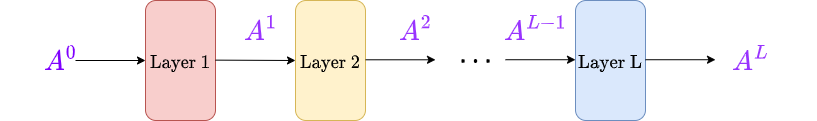
\includegraphics[width=140mm,scale=0.4]{images/nn_images/all_layers.png}
        \end{figure}
        
        Again, we see that the \textbf{output} of layer $\ell$ is the \textbf{input} of layer $\ell+1$.\\
        
        \begin{concept}
            Each layer \vocab{feeds} into the next layer.
            
            $A^\ell$ is the \purp{output} of layer $\ell$, and the \purp{input} of layer $\ell+1$.
            
            This means that the \purp{output} dimension must \gren{match} the next \purp{input} dimension.
            
            \begin{equation*}
                \overbrace{
                    n^\ell
                }^{\text{Output}}
                =
                \overbrace{
                    m^{\ell+1}
                }^{\text{Output}}
            \end{equation*}
            
            And the \vocab{dimension} of $A^\ell$ is $(n^\ell \times 1) = (m^{\ell+1} \times 1)$.
        \end{concept}
        
    \subsection*{Our Complete Neural Network}
    
        We can break our layers into components, so we can see the functions involved. 
        
        With this, we build our final neural network:
        
        \begin{figure}[H]
            \centering
            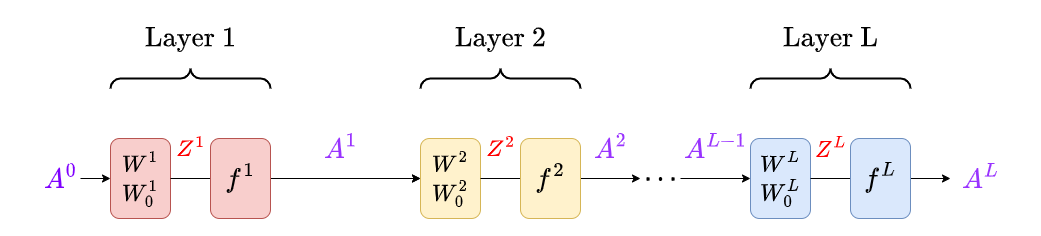
\includegraphics[width=140mm,scale=0.4]{images/nn_images/final_neural_network.png}
        \end{figure}
        
        With this, we can see how each layer is \textbf{related} to each other: as we \textbf{mentioned}, the \textbf{output} of one layer is the \textbf{input} of the next layer.
        
        Here is the computation we do for layer $\ell$:\\
        
        \begin{kequation}
            The calculations done by layer $\ell$ are given by
            
            \begin{equation*}
                \blu{Z^\ell} = (\blu{W^\ell})^T \red{A^{\ell-1}} + \blu{W_0^\ell} 
            \end{equation*}
            
            and
            
            \begin{equation*}
                \blu{A^\ell} = f(\blu{Z^\ell})
            \end{equation*}
            
            Which combine into:
            
            \begin{equation*}
                \blu{A^\ell} = f(\blu{Z^\ell}) = 
                f  
                \Bigg( 
                    (\blu{W^\ell})^T \red{A^{\ell-1}} + \blu{W_0^\ell} 
                \Bigg)
            \end{equation*}
        \end{kequation}
        
        One more comment: a useful definition.\\
        
        \begin{definition}
            A \vocab{hidden layer} is any layer except for the \purp{last} one.
            
            It is called a "\gren{hidden}" layer because, if you're viewing the whole neural network based on
            
            \begin{itemize}
                \item \gren{Input} $x$ (first input)
                
                \item \gren{Output} $A^L$ (final output)
            \end{itemize}
            
            Then you can't see the \gren{output} of any of the layers except for the \purp{last} one.
        \end{definition}
        
        Sometimes you'll hear someone say that a hidden layer is any except the "\textbf{first} or \textbf{last}": by that, they mean you can view the \textbf{input} for the \textbf{first} layer, as well as the \textbf{output} for the \textbf{last} layer.

        But, when we're talking about \textbf{activation} functions (which we often are when we mention hidden layers, see below), we only care about whether the \textbf{output} is hidden!
        